\chapter{Implementation}
\section{Parser}

The parser was written in TypeScript. Although there are many frameworks that could have been used for lexical and syntactic analysis, these were not chosen. The main reason for this is that the parser was meant to be used within a website. In particular, the parser was expected to become an node package manager (NPM) package. Moreover, TML is quite a simple language, which made this task relatively easy and short.

\begin{figure}[htb]
    \centering
    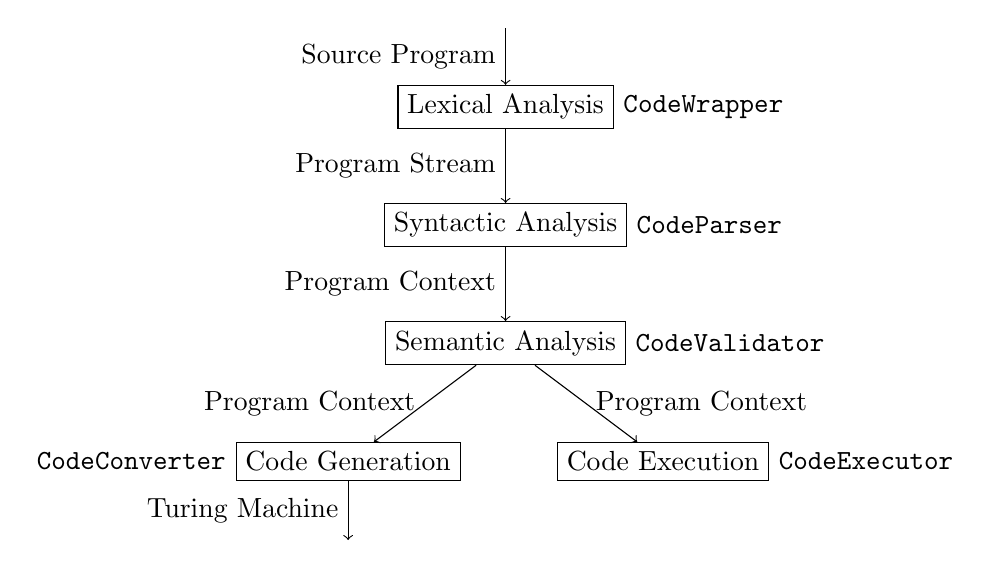
\begin{tikzpicture}
        \node[draw, label={0:\texttt{CodeWrapper}}] (CW) at (0, 0) {Lexical Analysis};
        \node[draw, label={0:\texttt{CodeParser}}] (CP) at (0, -1.5) {Syntactic Analysis};
        \node[draw, label={0:\texttt{CodeValidator}}] (CV) at (0, -3) {Semantic Analysis};
        \node[draw, label={180:\texttt{CodeConverter}}] (CC) at (-2, -4.5) {Code Generation};
        \node[draw, label={0:\texttt{CodeExecutor}}] (CE) at (2, -4.5) {Code Execution};

        \draw[->] (0, 1) -- node[left] {Source Program} (CW);
        \draw[->] (CW) -- node[left] {Program Stream} (CP);
        \draw[->] (CP) -- node[left] {Program Context} (CV);
        \draw[->] (CV) -- node[left] {Program Context} (CC);
        \draw[->] (CV) -- node[right] {Program Context} (CE);
        \draw[->] (CC) -- node[left] {Turing Machine} (-2, -5.5);
    \end{tikzpicture}
    \caption{The parsing process. The process is given inside the box. The class used to achieve the process is given in label, outside of the box. The flow of data is also shown.}
    \label{fig:parsing_process}
\end{figure}

The entire parsing process is summarised in Figure \ref{fig:parsing_process}.


\subsection{Lexical Analysis}

During lexical analysis, a stream of source code was produced. Although the source code was not enriched into tokens, the position of the code was tracked. This was to ensure that, in case of an error, the right section of code could be highlighted. This is done using the class \texttt{CodeWrapper}. 

To produce a stream of tokens, the \emph{iterator design pattern} was used. The iterator design pattern allows us to get the current value from a collection in a way that abstracts the data structure (\cite{gamma1995design}). In particular, the pattern was used to abstract the string representation of the source code and return a single entry from the code at a time. 

\subsection{Syntactic Analysis}
\begin{figure}[htb]
    \centering
    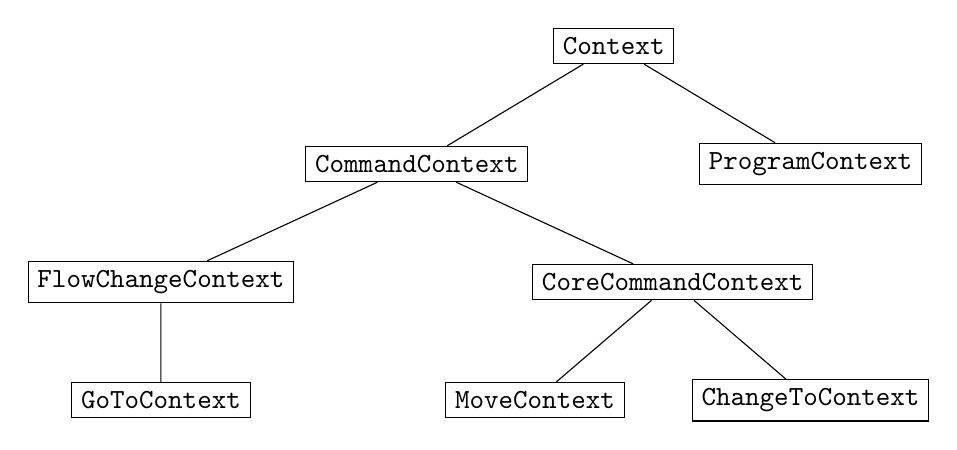
\begin{tikzpicture}[
        level 1/.style={sibling distance=5cm},
        level 2/.style={sibling distance=6.5cm},
        level 3/.style={sibling distance=3.5cm},
    ]
        \node[draw] {\texttt{Context}}
        child {
            node[draw] {\texttt{CommandContext}}
            child {
                node[draw] {\texttt{FlowChangeContext}}
                child {
                    node[draw] {\texttt{GoToContext}}
                }
            }
            child {
                node[draw] {\texttt{CoreCommandContext}}
                child {
                    node[draw] {\texttt{MoveContext}}
                }
                child {
                    node[draw] {\texttt{ChangeToContext}}
                }
            }
        }
        child {
            node[draw] {\texttt{ProgramContext}}
        };
    \end{tikzpicture}
    \caption{A snippet of the \texttt{Context} class hierarchy. All the non-leaf classes are abstract.}
    \label{fig:context_hierarchy}
\end{figure}

Next, the code is parsed. This is done using the class \texttt{CodeParser}. 

The result of the parsing is a \texttt{ProgramContext}, which represents the root of the AST. Subclasses of the \texttt{Context} class are used to represent different statements in the class, such as \texttt{MoveContext} for \textit{move} commands and \texttt{GoToContext} for \textit{goto} commands. A snippet of the class hierarchy for \texttt{Context} is shown in Figure \ref{fig:context_hierarchy}.

The parsing process results in the construction of the AST, such as the one in Figure \ref{fig:TML_AST}. To descend to a child, we make use of the instance fields. For instance, \texttt{ProgramContext} has the following fields:
\begin{itemize}
    \item \texttt{alphabet} for \texttt{AlphabetContext}; and
    \item \texttt{modules} for an array of \texttt{ModuleContext}.
\end{itemize}

The parser is recursive-descent, meaning that we delegate the parsing procedure to a method that parses a specific construct. For example, \texttt{parseModule} parses a \textit{module}, while \texttt{parseIf} parses an \textit{if} command. A snippet of the method \texttt{parseProgram} is given below.
\begin{lstlisting}[language=TypeScript]
parseProgram():ProgramContext {
    var alphabet:AlphabetContext = parseAlphabet();
    
    var modules:ModuleContext[] = [];
    while (this.code.moveNext()) {
        modules.add(parseModule());
    }
    
    return new ProgramContext(position, alphabet, modules);
}
\end{lstlisting}
Note that the code given above is simplified from the actual implementation.

\subsection{Semantic Analysis}
During semantic analysis, we traverse the AST using the \emph{visitor design pattern}. The visitor design pattern allows us to construct the same method for a class hierarchy without making changes to the classes (\cite{gamma1995design}). In this case, we want to create a method to validate each \texttt{Context}. Moreover, the semantic analysis is conducted by the class \texttt{CodeValidator}, which implements \texttt{CodeVisitor} to accommodate the visitor design pattern.

To allow for visitor design pattern, a concrete \texttt{Context} class implements the method \texttt{visit}. Each concrete class makes use of the right method from the abstract \texttt{CodeVisitor} class. We illustrate this with an example. Consider the following snippet of \texttt{GoToContext}.
\begin{lstlisting}[language=TypeScript]
class GoToContext extends FlowChangeContext {    
    identifier:string;
    
    visit<T>(visitor:CodeVisitor<T>):T {
        return visitor.visitGoTo(this);
    }

    // ... other methods for goto context
}
\end{lstlisting}
    Each \texttt{Context} class makes use of the right visitor method given in \texttt{CodeVisitor}. Now, in the \texttt{CodeValidator} class, we can define the following method that `visits' a \textit{goto} statement and validates it.
\begin{lstlisting}[language=TypeScript]
class CodeValidator extends CodeVisitor<boolean> {
    visit(context:Context):boolean {
        return context.visit(this);
    }
    
    // validate that the goto identifier a module name
    visitGoTo(gotoContext:GoToContext):boolean {
        if (!moduleNames.contains(gotoContext.identifier)) {
            throw new CodeError("Undefined name- " + identifier);
        }

        return true;
    }

    // ... other visitor methods
}
\end{lstlisting}
To run the \texttt{CodeValidator}, we visit \texttt{ProgramContext}.

When traversing the AST, we typically want to aggregate the result or share it with the parent. For this reason, we typically return a specific type of values within each visit method. To allow any type to be returned, the class \texttt{CodeVisitor} has a type parameter that represents the return type of each \texttt{visit} method.

In \texttt{CodeValidator}, we return \texttt{boolean} values. In particular, we return \texttt{true} if a block has a \textit{flow} command. This data is used in containers that have multiple blocks, such as a module. We throw an error if a non-final block has a \textit{flow} command. In the example code above, a block with a \textit{goto} command returns \texttt{true} since it is a \textit{flow} command. 

% A disadvantage of using the visitor design pattern is that the return value might not make sense in all subclasses. For instance, the value returned by \texttt{ProgramContext} does not make a difference in the validation process. There are other constructs as well for which the value does not make sense. In all these cases, to adhere to the pattern, we return \texttt{true}.

The advantage of using the visitor design pattern is that we have a way of traversing the AST without altering any of the \texttt{Context} classes; we can just construct a \texttt{Visitor} class. However, if we wanted to add another \texttt{Context} subclass, then we would need to amend all the \texttt{Visitor} classes. We expect the language to be pretty static, so this is perfectly fine in our case.


\subsection{TM Generation}
Next, we convert the AST into a TM. 

The TM is implemented in the class \texttt{TuringMachine} and mimics the definition of a TM. In particular, a TM is composed of many instances of \texttt{TMState}, which represent states within a TM. A TM state instance has a method \texttt{transition} that takes in a letter and returns the transition data, as a \texttt{TMChange}. A \texttt{TMChange} shows:
\begin{itemize}
    \item the next state value;
    \item the direction to move; and
    \item the value the tapehead value will become.
\end{itemize}

We traverse the AST using the visitor design pattern. Initially, we define the TM and add relevant states and transitions during the traversal. 

The visitor methods return the label of the next state, if applicable. This is defined in a very complex manner, depending on whether we have an \textit{if} or a \textit{while} command, or none at all! Hence, we delegate this responsibility from a \textit{switch} block to the relevant case command.

\subsection{Code and TM Execution}
Finally, a validated program can be executed using \texttt{CodeExecutor}. This class follows the iterator design pattern. In particular, we can make use of the method \texttt{execute} to run one step in execution. This method returns \texttt{false} if and only if execution has not terminated. The steps of execution are defined precisely in the language specification, given in the appendix.

Unlike the previous two stages, code execution does not make use of the visitor design pattern. This is because we do not need to traverse the AST in one go to convert the program. Instead, it makes more sense to use the iterator design pattern- this supports execution one step at a time.

TM execution has been implemented in the class \texttt{TMExecutor}. This also makes use of the iterator design pattern and supports execution one step at a time. The definition of TM execution is given in the background section.

\section{Product}
% Screenshots of the website homepage, documentation and error pages are given in the appendix. 

Due to the complex nature of the website, it made use of many APIs.

\subsection{Website Framework}

Initially, 3 frameworks were considered to implement the website:
\begin{itemize}
    \item the \emph{Webpack} framework - it has little overhead, allows for a lot of flexibility, but does not directly provide components (such as toolbar and drawer) or support state management (\cite{webpack});
    \item the \emph{React} framework- it has significantly more overhead than Webpack, but it also provides a rich collection of components and supports state management directly (\cite{react});
    \item the \emph{Angular} framework- it has even more overhead than React, but, like React, it has a rich collection of components and supports state management (\cite{angular}).
\end{itemize}

\emph{State management} was an important consideration when choosing the framework since the website tracks many states, such as the value of the editor and the current TM. Managing state manually would increase the complexity of the project, and could easily be avoided by choosing the right framework. For this reason, webpack was not chosen.

Both React and Angular would have been equally good choices for the project. React was chosen as there are more APIs that readily integrate with React compared to Angular, including some of the APIs used in this project. This is true since React is more widely used than Angular (\cite{react_v_angular}). The React framework supports coding in either JavaScript or TypeScript. The project made use of the TypeScript version for type safety.

\subsection{Editor}

The editor feature was implemented using the \emph{monaco} API. The API was chosen since it integrates well with React and provides many features (\cite{monaco}). The features include:
\begin{itemize}
    \item syntax highlighting with different priorities (e.g. an error gets a high priority while code execution gets a low priority);
    \item the ability to easily set and get the current value; along with
    \item numerous customisations to the editor, such as as changing the font size, setting an editor theme and showing/hiding line numbers- these are all features that a user can configure within the website.
\end{itemize}
Moreover, the monaco editor was chosen since it has the same look as Visual Studio (VS) Code, and shares many functionalities with the IDE. A developer survey in 2022 found that VS Code is the most popular code editor among 70 000 developers (\cite{stack_overflow}).

\subsection{FSM Generation}
\begin{figure}[htb]
    \centering
    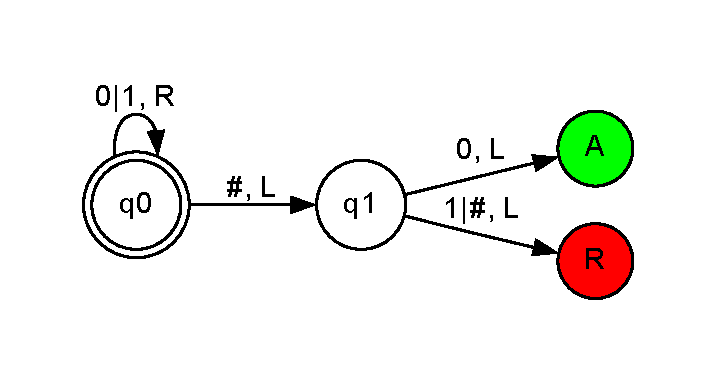
\includegraphics[scale=0.7]{images/graphviz_isDiv2.pdf}
    \caption{The graphviz rendering of the directed graph \texttt{isDiv2}.}
    \label{fig:graphviz_isDiv2}
\end{figure}

The FSM representation of the TM is created using the \emph{graphviz} framework. The API makes use of the \emph{DOT} notation (\cite{graphviz}). The DOT notation represents graphs in text by listing their nodes and edges (\cite{dot}). A graph in DOT notation is given below:
\begin{lstlisting}[language=DOT]
digraph isDiv2 {
    node [shape = "doublecircle"]; q0;
    node [shape = "circle"]; q1;
    node [style = "filled", fillcolor = "green"]; A;
    node [style = "filled", fillcolor = "red"]; R;
    q0 -> q0 [label = "0|1, R"];
    q0 -> q1 [label = "#, L"];
    q1 -> A [label = "0, L"];
    q1 -> R [label = "1|#, L"];
}
\end{lstlisting}
This graph represents the FSM representation of a TM. In this graph:
\begin{itemize}
    \item the keyword \texttt{digraph} implies that the graph is directed;
    \item the keyword \texttt{node} creates a state; and
    \item the arrow symbol (\texttt{->}) constructs edges between 2 states.
\end{itemize}
Nodes and edges take optional parameters within square brackets that allows them to be customised.

Using the graphviz API, the graph in DOT notation can be rendered in the website- the result for the directed graph \texttt{isDiv2} is given in Figure \ref{fig:graphviz_isDiv2}. Note that the figure was produced with some extra formatting code that is not shown.

We convert a TM to DOT notation as follows:
\begin{itemize}
    \item we set the default formatting of a node to be a circle (similar to code in line 3 of the example);
    \item we list the initial state \texttt{q0}, the accept state \texttt{A} and the reject state \texttt{R}, with the right formatting (like in lines 2, 4 and 5); and 
    \item we then list all the edges and label them with the corresponding transition (like in lines 6-9).
\end{itemize}

The advantage of using the graphviz package is that it can produce a well-formatted FSM. Initially, the graph was rendered by placing the states in order of its label, similar to Figure \ref{fig:bad_FSM}. The user would be able to drag the states and hence achieve a more reasonable placement. However, there was time to make use of the graphviz package later in the project, and so the implementation was changed. Now, the user is unable to drag the states, but this should not be necessary as the states are already well-placed!

\subsection{TM Formal Definition Conversion}
The formal definition of a TM is constructed quite naturally by using the class \texttt{TuringMachine}- we can look at the \texttt{transition} function to find an object of type \texttt{TMChange}. The values are shown to the user in a table like the one in Figure \ref{tbl:table_isDiv2}.

The text in the table is constructed using the \emph{MathJax} framework. This framework compiles raw code in LaTeX and renders it as an SVG.

\subsection{Tape Execution}

The tape entries were implemented as SVG elements. These were constructed using the \emph{d3} API. To illustrate tape execution, we make use of the animation subpackage in d3. This is used to move the tape left or right, and to change its value. 

During execution, we also highlight the current block being executed. Moreover, if the TM panel has been rendered, we highlight the current state and transition in the FSM representation. To keep track of these values, we execute the tape on both the TML program (using \texttt{CodeExecutor}) and its corresponding TM (using \texttt{TMExecutor}). We make use of the d3 API here as well to animate the change in current block/state.
